
%(BEGIN_QUESTION)
% Copyright 2012, Tony R. Kuphaldt, released under the Creative Commons Attribution License (v 1.0)
% This means you may do almost anything with this work of mine, so long as you give me proper credit

Shade the area(s) on this graph representing the following integral (assuming each horizontal and vertical division on the graph has an incremental value of 1):

$$\includegraphics[width=15.5cm]{i01919x01.eps}$$

$$\int_{-7}^{0} (z - y) \> dx$$

Also, determine whether the numerical value of this integral is {\it positive} or {\it negative}.

\underbar{file i01919}
%(END_QUESTION)





%(BEGIN_ANSWER)

This integral has a {\it positive} value:

$$\includegraphics[width=15.5cm]{i01919x02.eps}$$

From $x = -7$ to approximately $x = -1.75$, the integral accumulates a positive value because it has positive $dx$ increments and $z$ is larger than $y$.  From approximately $x = -1.75$ to $x = 0$ the integral accumulates a negative value because $y$ is larger than $z$ (a negative integrand) while $dx$ increments still remain positive.  Overall, the positive area is greater than the negative area, and so the integral from $x = -7$ to $x = 0$ has a net positive value.

%(END_ANSWER)





%(BEGIN_NOTES)


%INDEX% Mathematics, calculus: integral (defined in a graphical sense)

%(END_NOTES)


